\documentclass[fontsize=12pt]{scrartcl} % A4 paper and 11pt font size
\usepackage[utf8]{inputenc} % for french
\usepackage[T1]{fontenc} % Use 8-bit encoding that has 256 glyphs
\usepackage[english]{babel} % English language/hyphenation
\usepackage{amsmath,amsfonts,amsthm} % Math packages
\usepackage{amssymb}
\usepackage{url}

\usepackage{float}
\usepackage{graphicx}

\usepackage{listings}
\usepackage{courier}

% parameters for listings
\usepackage{color}
\definecolor{mygrey}{rgb}{0.96,0.96,0.96}
\lstset{
  tabsize=4,
  basicstyle=\ttfamily,
  backgroundcolor=\color{mygrey},
  captionpos=b,
  breaklines=true
}

%\fontsize{16pt}

\usepackage{lipsum} % Used for inserting dummy 'Lorem ipsum' text into the template
\usepackage{hyperref}

\usepackage{sectsty} % Allows customizing section commands
\allsectionsfont{\centering \normalfont\scshape} % Make all sections centered, the default font and small caps

\usepackage{eurosym}

\usepackage{fancyhdr} % Custom headers and footers
\pagestyle{fancyplain} % Makes all pages in the document conform to the custom headers and footers
\fancyhead{} % No page header - if you want one, create it in the same way as the footers below
\fancyfoot[L]{} % Empty left footer
\fancyfoot[C]{} % Empty center footer
\fancyfoot[R]{\thepage} % Page numbering for right footer
\renewcommand{\headrulewidth}{0pt} % Remove header underlines
\renewcommand{\footrulewidth}{0pt} % Remove footer underlines
\setlength{\headheight}{13.6pt} % Customize the height of the header

\numberwithin{equation}{section} % Number equations within sections (i.e. 1.1, 1.2, 2.1, 2.2 instead of 1, 2, 3, 4)
\numberwithin{figure}{section} % Number figures within sections (i.e. 1.1, 1.2, 2.1, 2.2 instead of 1, 2, 3, 4)
\numberwithin{table}{section} % Number tables within sections (i.e. 1.1, 1.2, 2.1, 2.2 instead of 1, 2, 3, 4)

\setlength\parindent{2em} % Removes all indentation from paragraphs - comment this line for an assignment with lots of text
%\setlength{\parskip}{1em}

%\renewcommand{\baselinestretch}{1.5}

%----------------------------------------------------------------------------------------
%	TITLE SECTION
%----------------------------------------------------------------------------------------

\newcommand{\horrule}[1]{\rule{\linewidth}{#1}} % Create horizontal rule command with 1 argument of height

\title{	
\normalfont \normalsize 
\textsc{UJM (Saint-Etienne) // GRAME-CNCM (Lyon) // Gipsa-Lab (Grenoble)} \\ [25pt] % Your university, school and/or department name(s)
\horrule{0.5pt} \\[0.4cm] % Thin top horizontal rule
\huge Application for the Organization of the 18th Sound and Music Computing Conference and Summer School \\ % The assignment title
\horrule{2pt} \\[0.5cm] % Thick bottom horizontal rule
}

\date{} % Today's date or a custom date

\begin{document}

\maketitle % Print the title

In this draft document, we address the various points regarding the organization of the 2021 Sound and Music Computing (SMC) Conference and Summer School in Saint-Étienne (France). The time frame being still very large at this point, this proposal will likely be prompt to adjustments in the future but should nonetheless give a clear idea of the project. 

\tableofcontents

% TODO: keynotes

\section{Context}

The SMC conference and the JIM\footnote{\textit{Journées de l'Informatique Musicale}} (French computer music conference) share a long common history since SMC was born from the union of the JIM and of the CIM\footnote{\textit{Colloqui di Informatica Musicale}} (the Italian counterpart of the JIM). In that context, we propose to organize a joint event between the JIM and SMC\footnote{Practically, this would mean that JIM would be replaced by SMC as this was done in 2004 in Paris and in 2006 in Marseille.} in Saint-Étienne (France) during the second half of June 2021. 

Saint-Étienne was nominated as ``City of Design'' as part of UNESCO's Creative Cities Network\footnote{\url{https://en.unesco.org/creative-cities/}} and has a long-standing tradition of supporting exploratory and contemporary art creation thanks to institutions such as the Contemporary Art Museum (``Musée d'Art Contemporain,'' one of the largest in France) and the Cité du design (``City of Design''). Hence, it is only natural that we propose the following theme for the conference: ``\textbf{Computer Music and Design}.'' Saint-Étienne is also characterized by its industrial heritage (i.e., coal mining, weapon industry, etc.) which left plethora of unusual spaces, which of whom are now used for art exhibits, residencies and performances.

Saint-Étienne is located at the heart of the Auvergne-Rhône-Alpes region which is home of multiple centers and institutions involved in the field of music technology and computer music. As such, we plan to unify forces by presenting a region-wide project involving multiple centers: the CIEREC (UJM, Saint-Étienne), GRAME-CNCM (Lyon), and Gipsa-Lab (Grenoble-INP, Grenoble).

\section{Organizing Committee and Partners}

The organization of SMC-21 will be the fruit of a collaboration between the CIEREC,\footnote{\textit{Centre Interdisciplinaire d'Études et de Recherches sur l'Expression Contemporaine}, Université Jean Monnet, Saint-Étienne: \url{https://www.univ-st-etienne.fr/fr/cierec.html}} GRAME-CNCM,\footnote{\textit{GRAME -- Centre National de Création Musicale}, Lyon: \url{https://faust.grame.fr}} and Gipsa-Lab\footnote{\textit{Grenoble Image Parole Signal Automatique}, Université Grenoble INP, Grenoble (France): \url{http://www.gipsa-lab.fr/}.} as well as multiple other partners:

\begin{itemize}
\item The Cité du design: \url{https://www.citedudesign.com}
\item Saint-Étienne Opera: \url{http://www.opera.saint-etienne.fr}
\item The FIL -- Scène de musique actuelle: \url{http://www.le-fil.com}
\item The Musée de la mine: \url{http://www.musee-mine.saint-etienne.fr/}
\item The Musée d'art moderne et contemporain: \url{https://mamc.saint-etienne.fr/} 
\item INSA\footnote{\textit{Institut National des Sciences Appliquées}} Lyon: \url{https://www.insa-lyon.fr}
\item Lyon University: \url{https://www.universite-lyon.fr/}
\item CCRMA,\footnote{\textit{Center for Computer Research in Music and Acoustics}} Stanford University: \url{https://ccrma.stanford.edu/~rmichon}
\end{itemize}

An overview of the current members of the organizing committee of the conference is provided in Table~\ref{tab:committee}. 

\begin{table}[!htbp]
  \begin{center}
    \begin{tabular}{c | c}
      \textbf{Name} & \textbf{Role} \\
      \hline
      \hline
      Romain Michon & Principal Chair/Organizer \\
      Laurent Pottier & Principal Chair/Organizer \\
      Yann Orlarey & Paper Chair \\
      Constantin Basica & Music Chair \\
      James Leonard & Summer School Chair \\
      Jérôme Villeneuve & Summer School Chair \\
    \end{tabular}
    \caption{SMC-21 Organizing Committee.}
    \label{tab:committee}
  \end{center}
\end{table}

\section{Dates}

While the exact dates of the conference haven't been defined yet, we aim for the second half of June 2021. This is a good time for us because finals will be over at this period and we know that July and August are often problematic for some members of the SMC community. Beside that, we plan to stick to the regular/standard SMC schedule for the review process and the summer school application, etc.

\section{Venues}
\label{sec:venues}

The conference will take place in a wide range of venues located throughout the city center of Saint-Étienne and accessible within a walking distance from each others. The scientific track and the summer school will both happen at the \textit{Cité du design} (see Figure~\ref{fig:cite}). Paper sessions will take place in the Main Auditorium (see Figure~\ref{fig:amphi}) which can host up to 300 people, and the summer school in the seminar room (see Figure~\ref{fig:summerSchool}) which can host up to 120 people. Poster sessions will be held in the \textit{Agora} (see Figure~\ref{fig:agora}) which will also be used for lunch breaks.

\begin{figure}[htpb]
\begin{center}
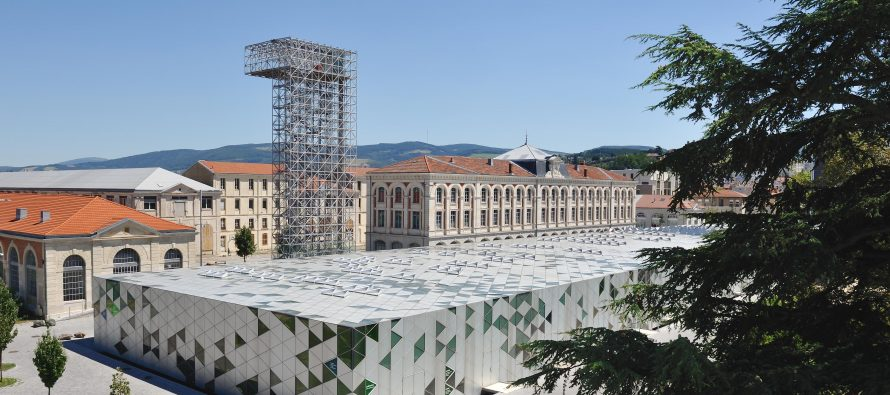
\includegraphics[width=\columnwidth{}]{img/cite.jpg}
\caption{The Cité du design.}
\label{fig:cite}
\end{center}
\end{figure}

\begin{figure}[htpb]
\begin{center}
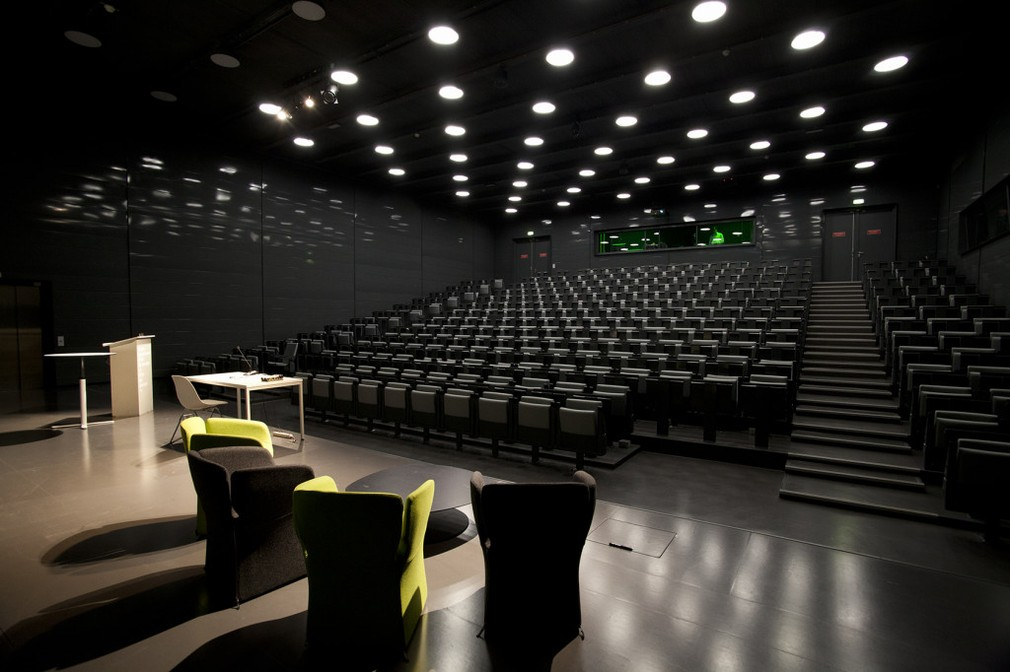
\includegraphics[scale=0.3]{img/amphi.jpg}
\caption{The Cité du design Auditorium: paper session venue.}
\label{fig:amphi}
\end{center}
\end{figure}

\begin{figure}[htpb]
\begin{center}
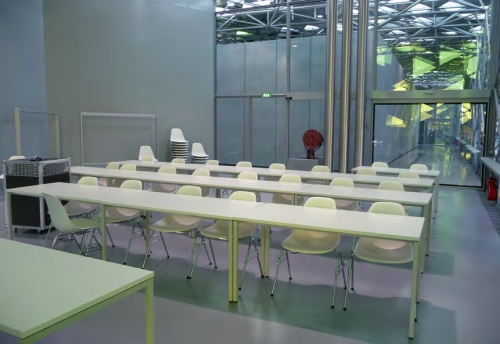
\includegraphics[scale=0.5]{img/summerSchool.jpg}
\caption{The Cité du design Seminar Room: Summer School venue.}
\label{fig:summerSchool}
\end{center}
\end{figure}

\begin{figure}[htpb]
\begin{center}
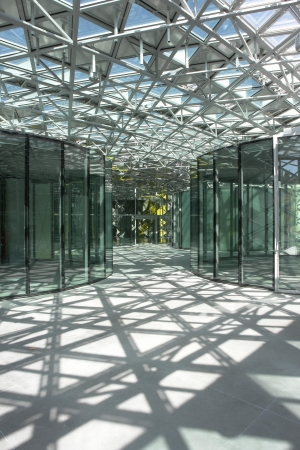
\includegraphics[scale=0.5]{img/agora.jpg}
\caption{The Cité du design Agora: poster session, lunch, and installations venue.}
\label{fig:agora}
\end{center}
\end{figure}

Saint-Étienne benefits from a wide panel of venues and unusual spaces for live music performance and interactive installations. The conference concerts will take place at:
\begin{itemize}
  \item The FIL (see Figure~\ref{fig:fil}): live/fixed media electronic music performance. This venue also hosts its own bar which makes it a great space for more casual performances with a standing audience.
  \item The Théâtre Copeau (see Figure~\ref{fig:copeau}): live contemporary music performance.
  \item The Maison de l'université (see Figure~\ref{fig:mume}): live/fixed media  performance.
\end{itemize}

\begin{figure}[htpb]
\begin{center}
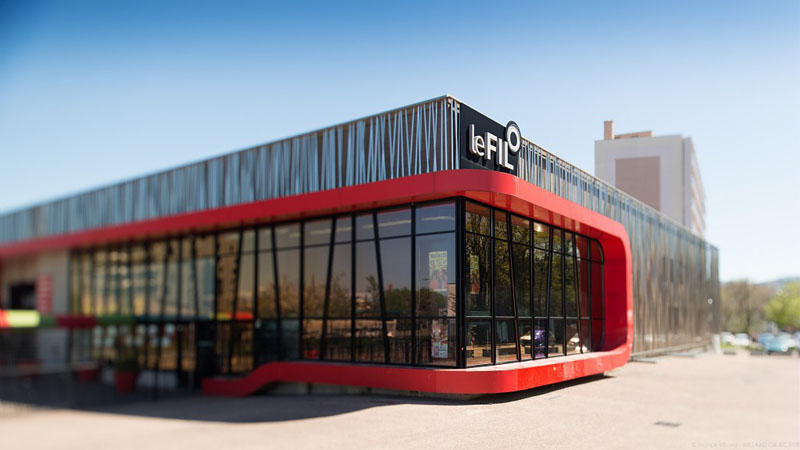
\includegraphics[scale=0.4]{img/fil.jpg}
\caption{The FIL: venue for live electronics concerts.}
\label{fig:fil}
\end{center}
\end{figure}

\begin{figure}[htpb]
\begin{center}
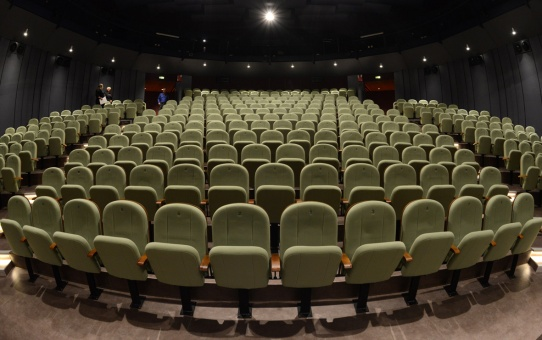
\includegraphics[scale=0.5]{img/copeau.jpeg}
\caption{The Théâtre Copeau: venue for live contemporary performance.}
\label{fig:copeau}
\end{center}
\end{figure}

\begin{figure}[htpb]
\begin{center}
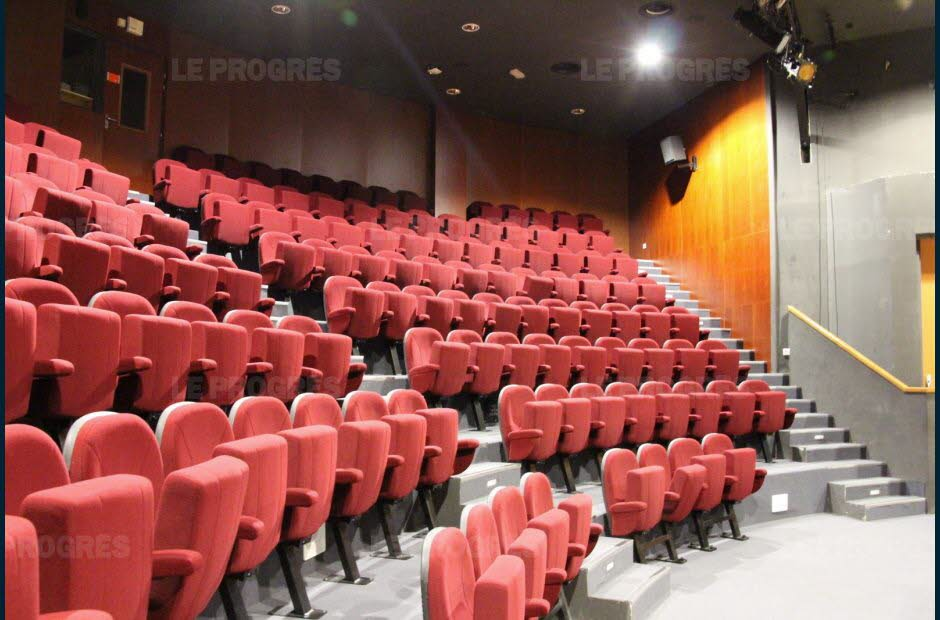
\includegraphics[scale=0.3]{img/mume.jpg}
\caption{The Maison de l'université auditorium: venue for live performance.}
\label{fig:mume}
\end{center}
\end{figure}

Various spaces will be available for interactive sound installations ranging from conventional exhibition halls such as the Agora of the Cité du design (see Figure~\ref{fig:agora}) to less conventional ones such as the Salle des pendus (``Hanged Men Room'': see Figure~\ref{fig:pendus}) at the Musée de la mine. 

\begin{figure}[htpb]
\begin{center}
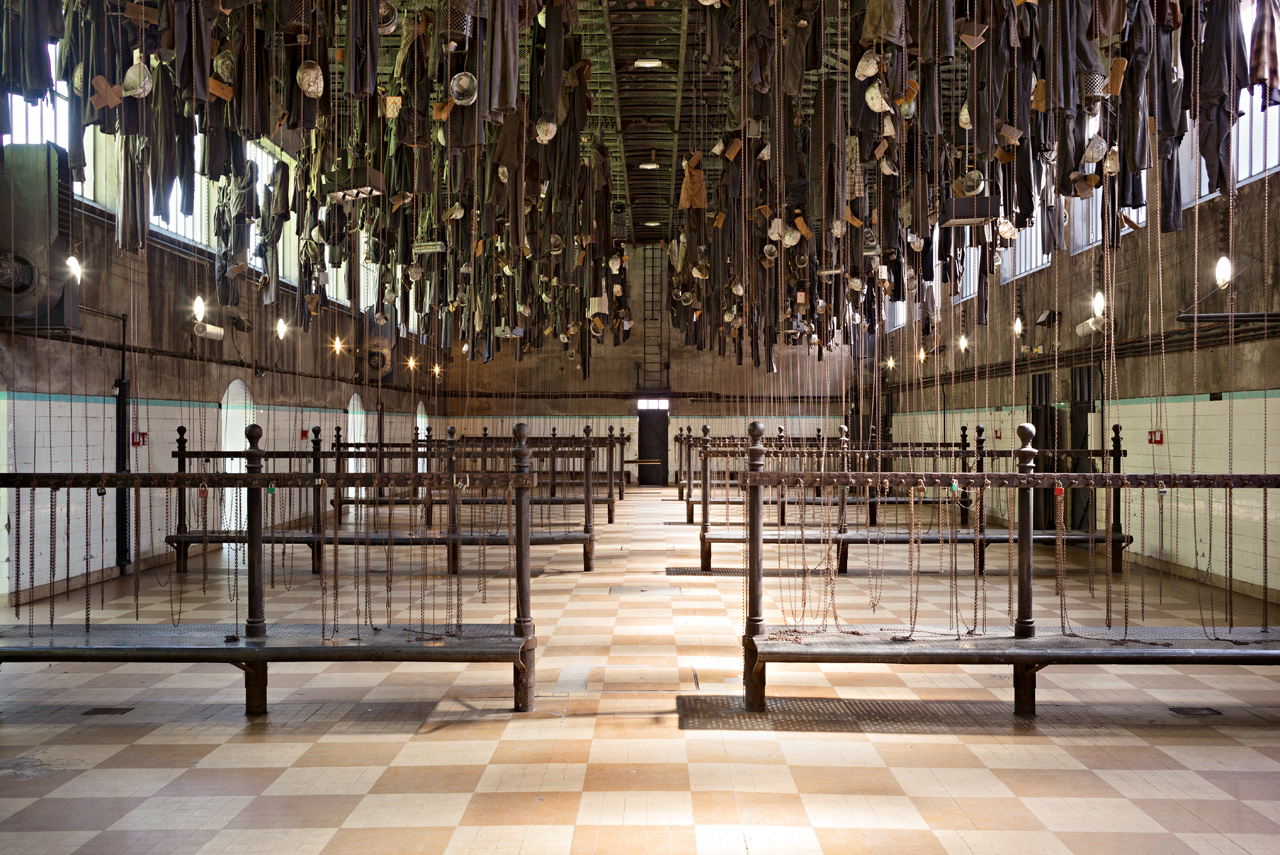
\includegraphics[scale=0.2]{img/pendus.jpg}
\caption{The Salle des pendus at the Musée de la mine: venue for installations and maybe performances.}
\label{fig:pendus}
\end{center}
\end{figure}

We're still working at finding more spaces for installations and concerts, but Saint-Étienne's industrial past offers plenty of opportunities for unconventional spaces.  

\section{Special Equipments and Resources}

GRAME-CNCM, Gipsa-Lab, and the UJM own a wide range of special equipments (e.g., interfaces, sound spatialisation systems such as acousmoniums, Ambisonics systems, etc.) that will be made available to composers during the conference for music submissions.

Similarly, we're trying to involve the superior conservatory of Lyon (CNSMD)\footnote{\url{http://www.cnsmd-lyon.fr/}} and the \textit{Ensemble Orchestral Contemporain}\footnote{\url{https://www.eoc.fr}} to offer the possibility to composers in the SMC community to collaborate with local ensembles and musicians. 

\section{Conference Schedule/Program}

SMC-21 will take place during the second half of June 2021. To the best of our knowledge, it currently doesn't conflict with any other conference in this field (i.e., ICMC, DAFx, NIME, ISMIR, etc.). It will follow the ``standard'' SMC schedule with 4 days of summer school followed by three days of conference. The summer school will feature 4 speakers and follow the general theme of the conference: ``Computer Music and Design.'' The conference will be single-track with paper presentations, demos, and poster sessions. We plan to have at least one concert for each day of the conference. Concerts will be organized by genres to provide the best space/equipment for each specific type of music (see \S\ref{sec:venues}): seated vs. standing, bar vs. formal, etc. Similarly, installations will be placed in various locations throughout the city (see \S\ref{sec:venues}). The conference will be punctuated by multiple social events such as the ``traditional'' conference banquet and opening reception.

We're currently investigating the idea of having a couple of side-concerts (that could perhaps take the form of a small festival) with invited ensembles and performances, but we're still working on this. We're also trying to see how the SMC music program could integrate to the cultural season of the various spaces associated to the conference to benefit from their communication networks and to reach a broader audience.

\section{Traveling to Saint-Étienne}

Saint-Étienne is located 65km south-east of Lyon and can be easily reached by plane or by train. The closest airport is Lyon Saint-Exupéry (LYS) which is connected to Saint-Étienne city center by 2 bus lines (one bus every hour). The trip between the airport and Saint-Étienne takes a bit more than an hour and is direct and non-stop. Saint-Étienne train station has a direct TGV train line to Paris (2h30). Finally, another good option is to fly to Paris Charles de Gaulle (CDG) and to take a train between the airport and Saint-Étienne (2h45).

\section{Financial Details/Budget}

We're in the very early stage of sketching the conference budget so we don't have much details to provide on this aspect at this point. We plan to apply for a couple of local grants to help fund the conference and to keep the registration fee as low as possible. Since SMC and the JIM will be the same event, we'll also automatically benefit from the 7000 \euro{} grant allocated by the AFIM\footnote{\textit{Association Française d'Informatique Musicale}} to organize this event. We hope to make the summer school free and to fund it with conference registrations. 

\section{Contacts}

\begin{itemize}
\item Romain Michon, GRAME-CNCM -- \texttt{michon@grame.fr}
\item Laurent Pottier, UJM -- \texttt{laurent.pottier@univ-st-etienne.fr}
\end{itemize}

\end{document}
